\section[Модели систем передачи информации]{Модели систем передачи информации с криптографической защитой}\index{канал связи!защищённый|(}\index{канал связи!открытый|(}
\selectlanguage{russian}

Простая модель системы передачи с криптографической защитой представлена на рис.~\ref{pic:model-simple}. На рисунке показаны легальный отправитель, легальный получатель, и криптоаналитик, который пытается нарушить безопасность информации в системе. Данные в системе передаются по открытому каналу связи. Можно также говорить, что криптографические преобразования на стороне отправителя и получателя позволили им создать \emph{защищённый канал связи} поверх открытого канала, как показано на рис.~\ref{pic:model-simple-with-channel}.

\begin{figure}[!thb]
	\centering
	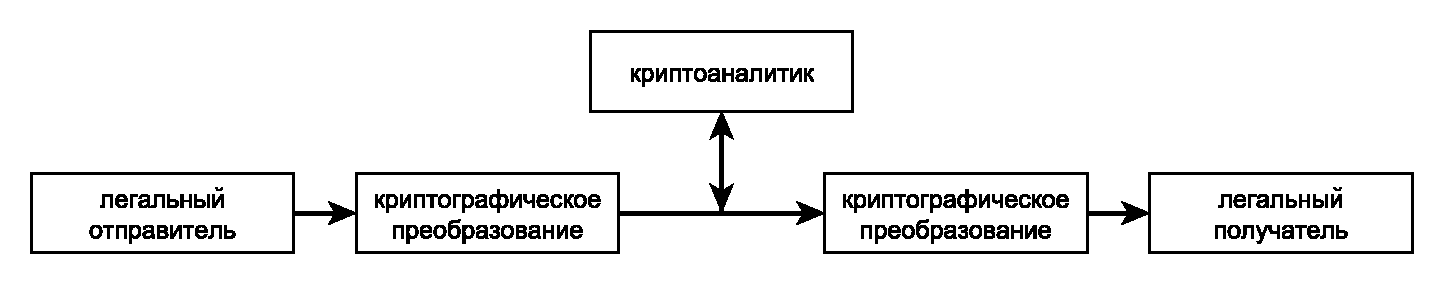
\includegraphics[width=1.0\textwidth]{pic/model-simple}
	\caption{Модель системы передачи информации с криптографической защитой по открытому каналу\label{pic:model-simple}}
\end{figure}

\begin{figure}[!thb]
	\centering
	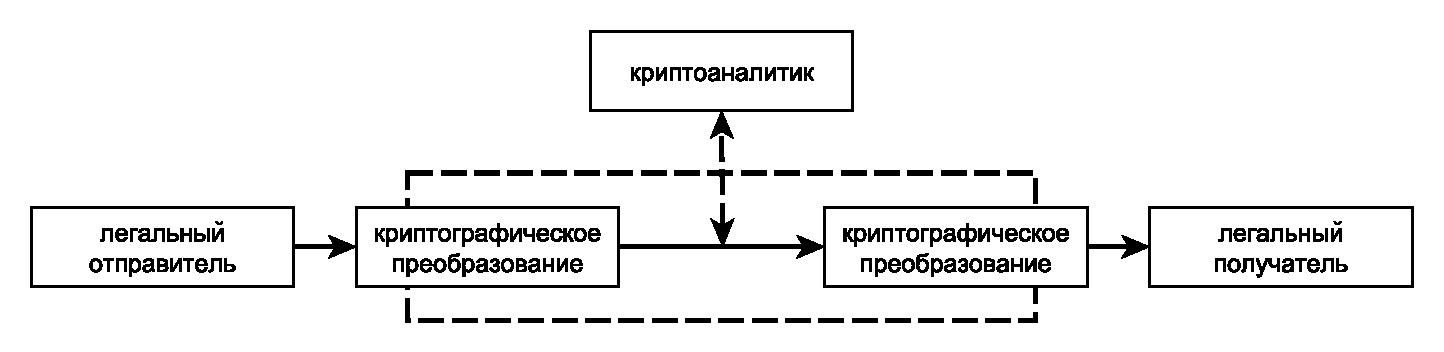
\includegraphics[width=1.0\textwidth]{pic/model-simple-with-channel}
	\caption{Открытый и защищённый каналы связи в модели системы передачи информации с криптографической защитой\label{pic:model-simple-with-channel}}
\end{figure}

Для обеспечения конфиденциальности информации используются криптографические системы с функцией шифрования. Пример системы с шифрованием показан на рис.~\ref{pic:model-cipher}.

\begin{figure}[!thb]
	\centering
	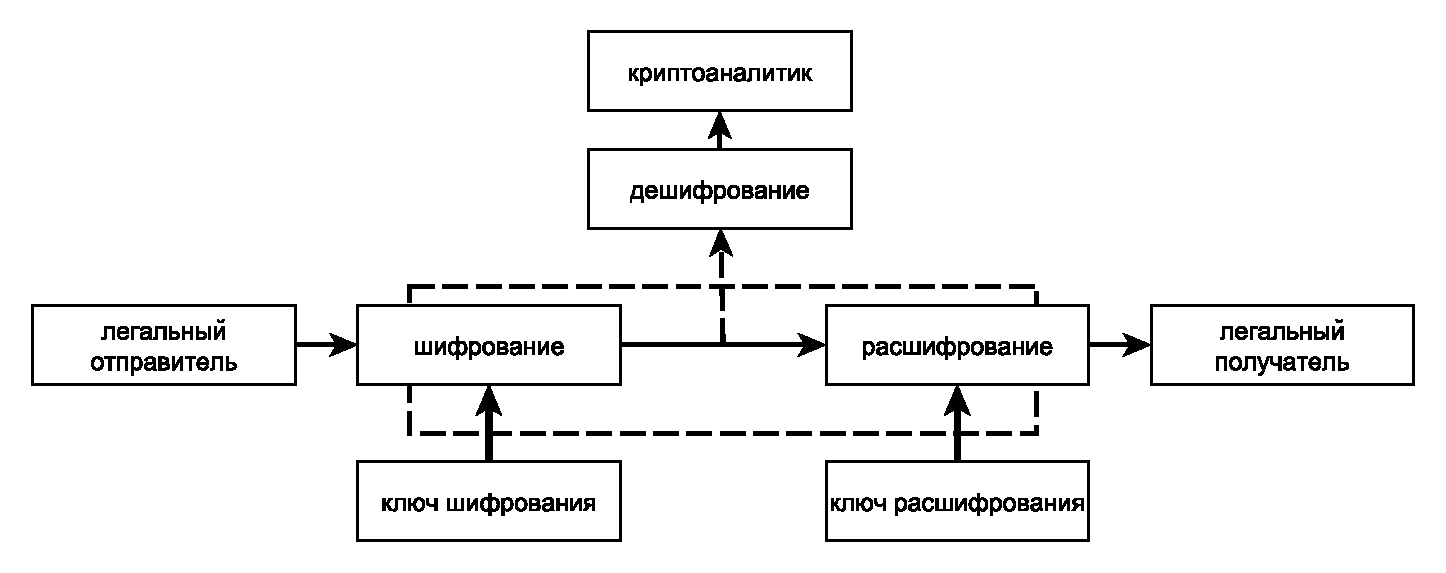
\includegraphics[width=1.0\textwidth]{pic/model-cipher}
	\caption{Модель системы передачи информации с шифрованием\label{pic:model-cipher}}
\end{figure}

Легальный отправитель \emph{шифрует} сообщение (\emph{открытый текст}\index{открытый текст}, \langen{plaintext}) с использованием \emph{ключа шифрования}\index{ключ!шифрования} (\langen{encryption key}) и передаёт зашифрованное сообщение (\emph{шифртекст}\index{шифртекст}, \langen{ciphertext, cyphertext} или \emph{шифрограмма}\index{шифрограмма}\footnote{Строго говоря, \emph{шифрограмма} -- это \emph{шифртекст} после его \emph{кодирования} для целей передачи по каналу связи.}) по открытому каналу связи. Легальный отправитель \emph{расшифровывает} сообщение, используя \emph{ключ расшифрования}\index{ключ!расшифрования}, в общем случае отличающийся от ключа шифрования. Нелегальный пользователь, называемый криптоаналитиком, пытается \emph{дешифровать}\footnote{Обратите внимание, что в англоязычной литературе словом <<\textit{decryption}>> обозначается и расшифрование, и дешифрование.} сообщение, не имея ключа расшифрования, то есть нарушить конфиденциальность передаваемой информации. Можно сказать, что функции шифрования и расшифрования вместе с конкретными ключами шифрования и расшифрования помогли легальным участникам системы установить защищённый канал связи, обеспечивающий конфиденциальность информации.

\emph{Шифрование} (\emph{зашифрование}) -- это обратимое преобразование данных, формирующее шифртекст из открытого текста. \emph{Расшифрование} -- операция, обратная к шифрованию. А вместе это \emph{шифр} -- криптографический метод, используемый для обеспечения конфиденциальности данных, включающий алгоритм зашифрования и алгоритм расшифрования.~\cite{GOST-89}

\emph{Шифр}\index{шифр} -- это множество обратимых функций отображения $E_{K_1}$\index{функция!шифрования} множества открытых текстов $\set{M}$ на множество шифртекстов $\set{C}$, зависящих от выбранного ключа шифрования $K_1$ из множества $\set{K}_E$, а также соответствующие им обратные функции расшифрования $D_{K_2}$, $\set{K}_D$, отображающие множество шифртекстов на множество открытых текстов:

\begin{equation}\label{eq:Encryption}\begin{array}{l}
	E_{k_1}, k_1 \in \set{K}_E: \set{M} \to \set{C}, \\
	D_{k_2}, k_2 \in \set{K}_D: \set{C} \to \set{M}, \\
	\forall k_1 \in \set{K}_E ~ \exists k_2 \in \set{K}_D: \\
	\forall m \in \set{M}: ~ E_{k_1} \left( m \right) = c, c \in \set{C}: \\
	D_{k_2} \left( c \right) = m.
\end{array}\end{equation}

Можно сказать, что шифрование -- это обратимая функция двух аргументов: сообщения и ключа. Обратимость -- основное условие корректности шифрования, по которому каждому зашифрованному сообщению $Y$ и ключу $K$ соответствует одно исходное сообщение $X$. Легальный пользователь $B$ (на приёмной стороне системы связи) получает сообщение $Y$ и осуществляет процедуру \emph{расшифрования}\index{расшифрование}.

Следует отличать \emph{шифрование} от \emph{кодирования}, будь то кодирование источника или канала. Под кодированием источника понимается преобразование информации для более компактного хранения, а под кодированием канала -- для повышения помехоустойчивости.

Модель системы передачи информации с обеспечением аутентичности передаваемых сообщений выглядит как показано на рис.~\ref{pic:model-auten}.

\begin{figure}[!thb]
	\centering
	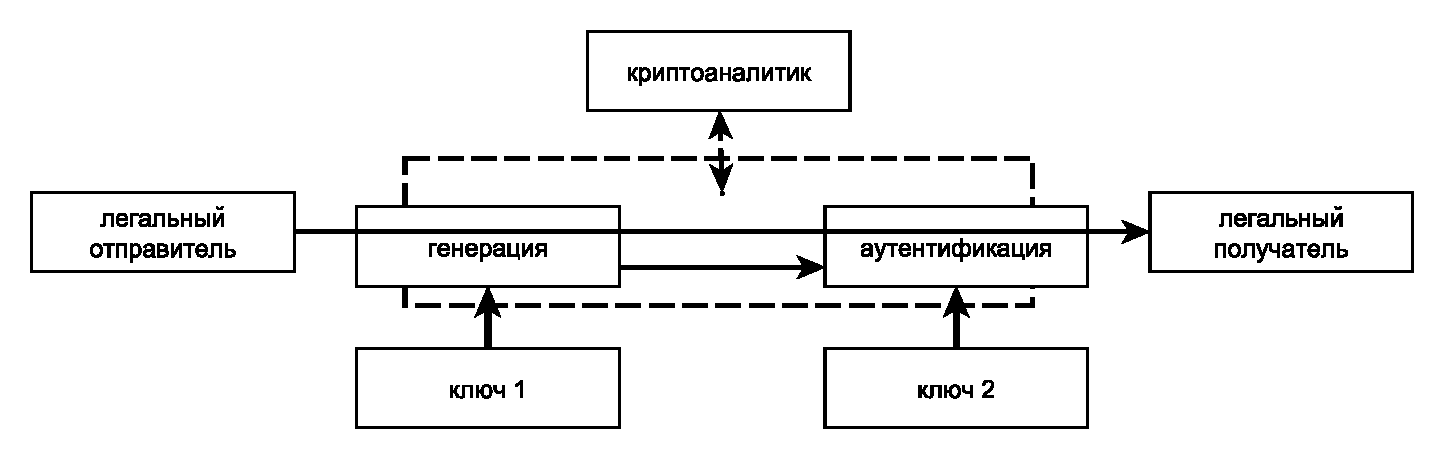
\includegraphics[width=1.0\textwidth]{pic/model-auten}
	\caption{Модель системы передачи информации с обеспечением аутентичности передаваемых сообщений\label{pic:model-auten}}
\end{figure}

В этой модели сообщение передаётся по открытому каналу связи без изменений (в открытом виде), однако вместе с сообщением от легального пользователя по тому же каналу связи передаётся дополнительная информация. Специальные криптографические методы позволяет гарантировать, что данную информацию может сформировать только легальный пользователь (или, в некоторых случаях, ещё и легальный получатель). Легальный получатель проверяет эту дополнительную информацию и убеждается, что сообщение пришло именно от легального отправителя и без изменений. Таким образом был организован защищённый канал связи с обеспечением аутентичности передаваемых сообщений. 

\index{канал связи!защищённый|)}\index{канал связи!открытый|)}
